\section{Ka/Ks Analysis}

\subsection{Introduction}

\subsection{Methods}

\subsubsection{Calculation of dN/dS}

Selective constraints on gene sequence evolution were estimated using the dN/dS statistic calculated for orthologous group multiple sequence alignments. 
Protein sequences were organized into ortholog groups according to OrthoDB v8 \textcolor{red}{TODO CITE}. Groups that did not have at least one sequence from each species were discarded.  For groups with 1-to-many and many-to-many orthologs, one protein sequence was chosen randomly with uniform weights from each species. Protein multiple sequence alignments were generated using Clustal Omega \textcolor{red}{TODO CITE} and used to inform CDS alignments with the codon-aware PAL2NAL alignment program \textcolor{red}{TODO CITE}.  The yn00 program from PAML v4.8 \textcolor{red}{TODO CITE} was used to calculate dN/dS ratios for each pairs of sequences in the aligned ortholog groups. 

\begin{figure}[H]
  \centering
  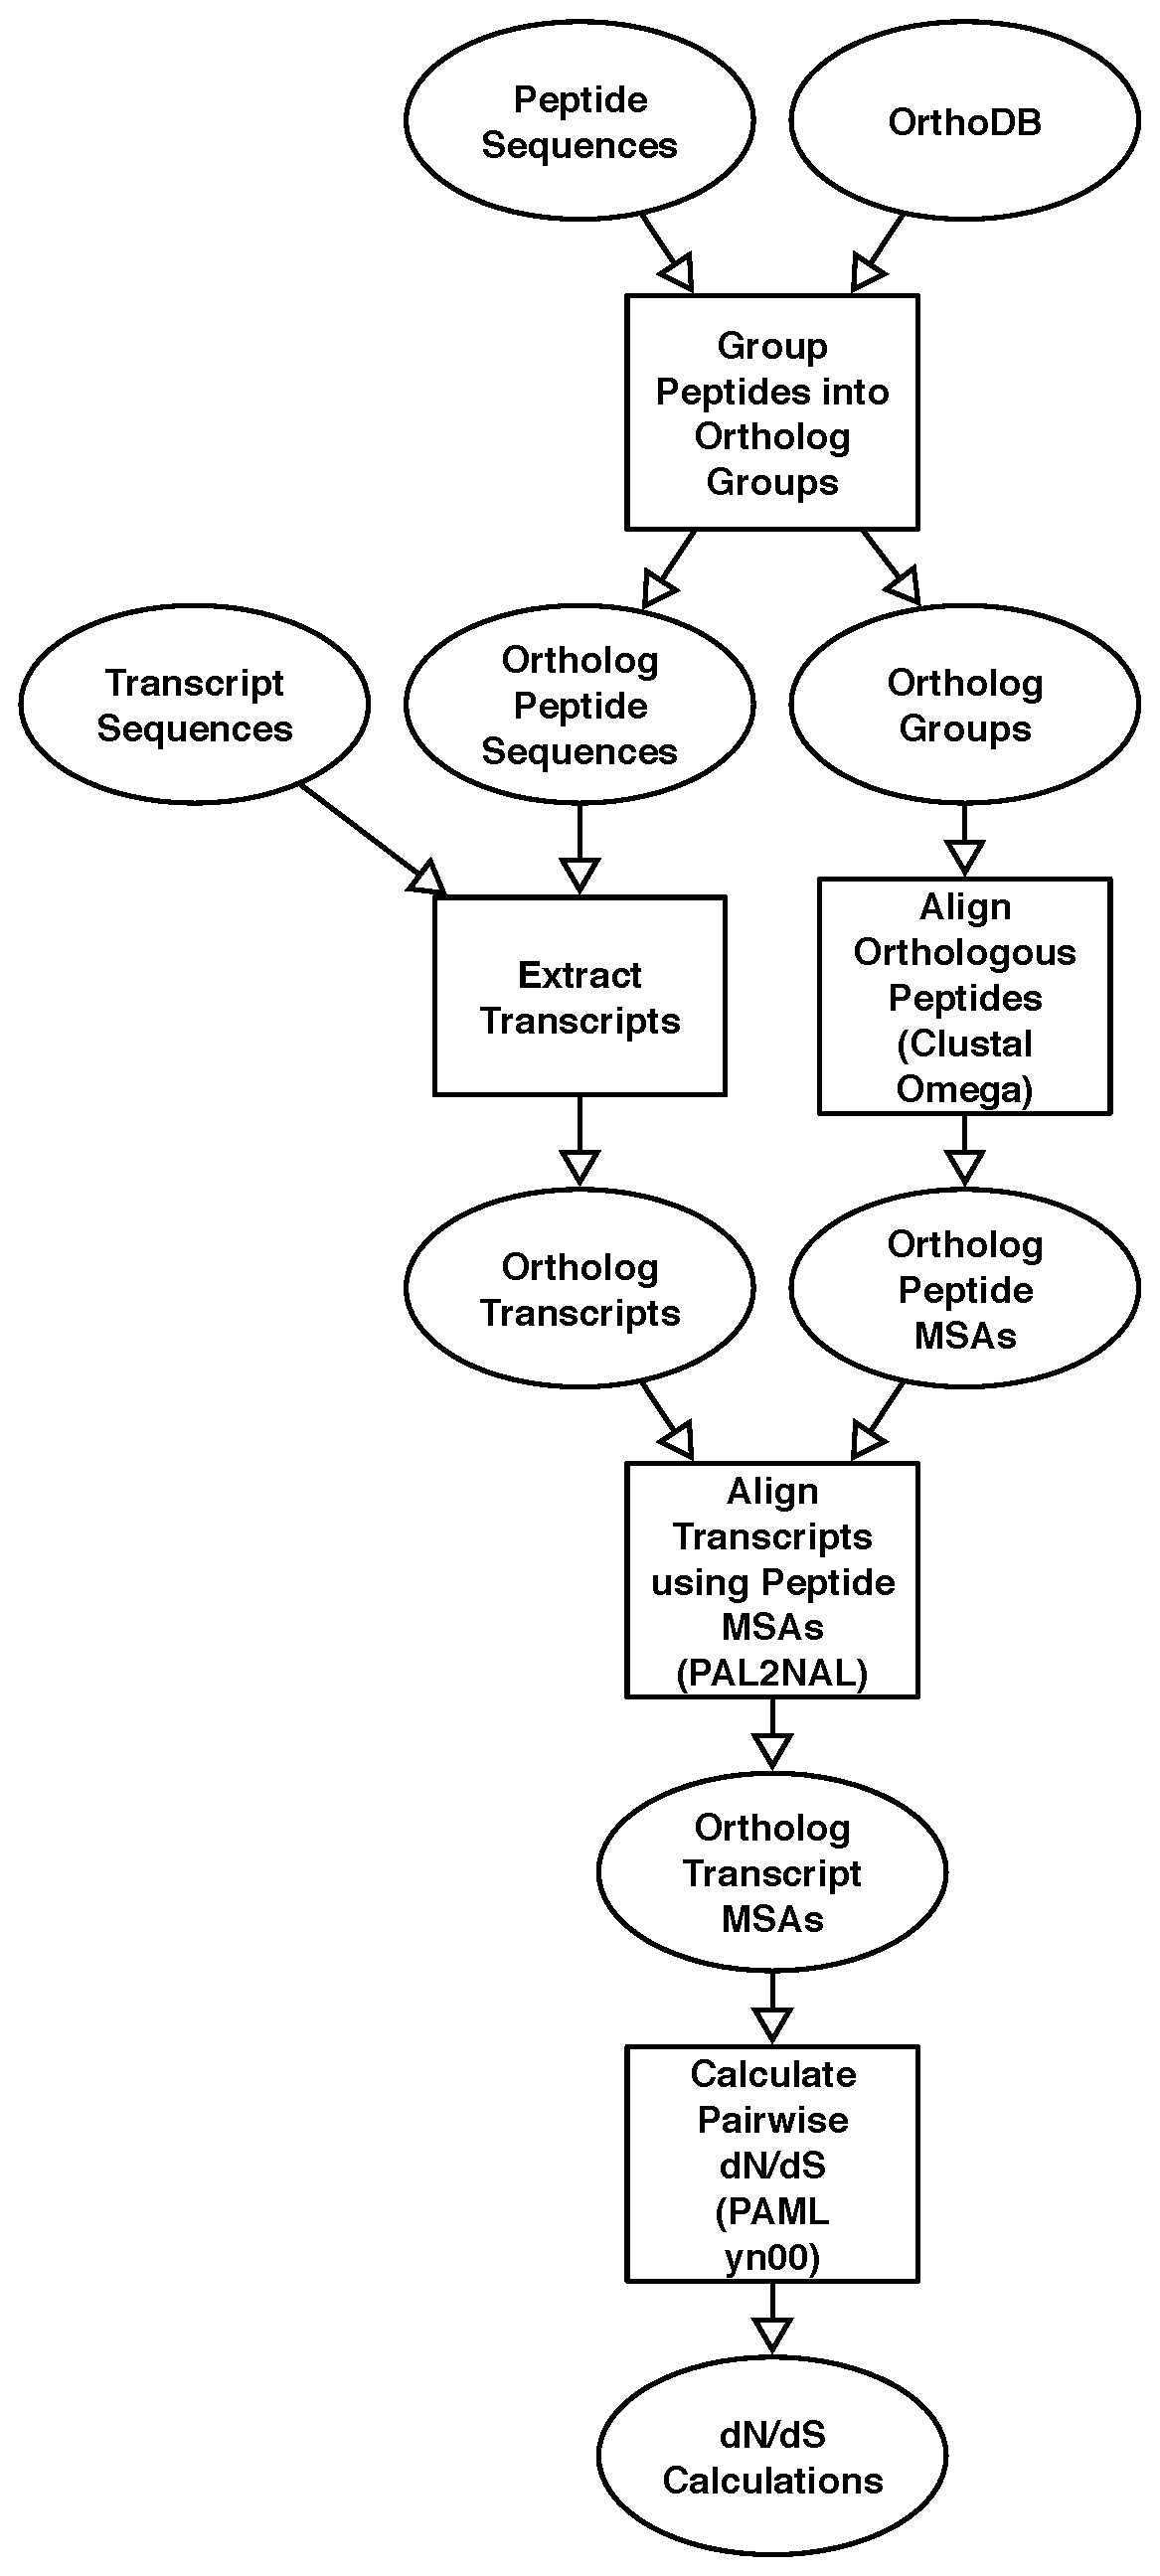
\includegraphics[width=0.5\textwidth]{figures/ka_ks/PAML_workflow}
  \caption{Workflow for Calculating dN/dS}
  \label{fig:ka-ks-workflow}
\end{figure}

\subsection{Results}

\subsubsection{Comparison of $d_N$/$d_S$ Distributions}
\begin{figure}[H]
  \centering
  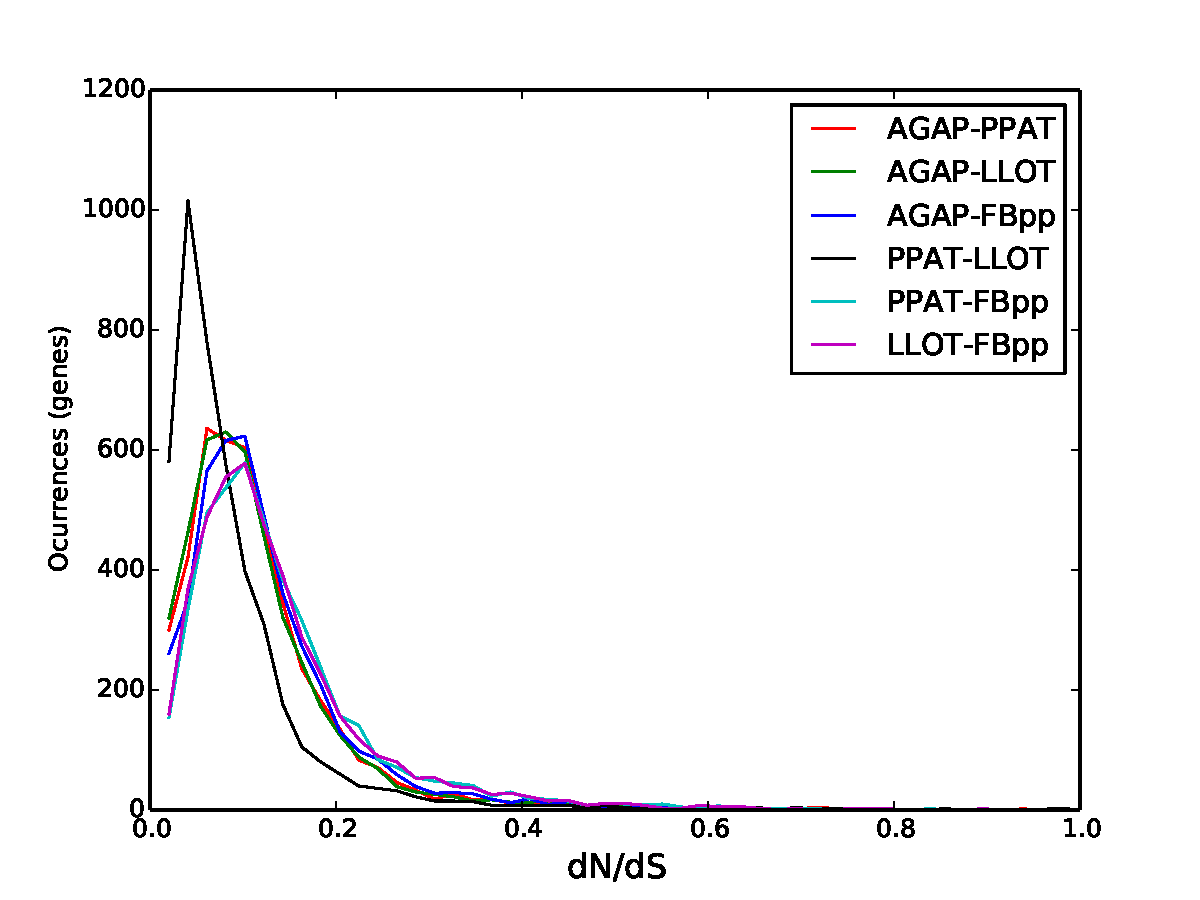
\includegraphics[width=0.5\textwidth]{figures/ka_ks/dN_dS}
  \caption{Distribution of dN/dS values}
  \label{fig:dnds-distr}
\end{figure}

\subsection{Analysis of Genes Undergoing Positive Selection}
\subsection{Discussion and Conclusion}